
\section{Introdução}
Nesta secção é apresentado o estado da arte dos projetos realizados durante o estágio na empresa CapTemp. Nessa ordem é apresentado o funcionamento do sistema do Nidus desenvolvido pela empresa CapTemp e a sua página de configuração e visualização. Na secção \ref{Página do Coletor de Dados Nidus} são apresentadas também as metodologias e tecnologias que o sistema implementa atualmente para a compressão das páginas que dão suporte ao sistema. Na secção \ref{nbiot} e \ref{kea} irá ser introduzido o plano inicial dos projetos a desenvolver e a base já existente tal como as tecnologias que estes irão utilizar. Na secção \ref{solucoesDisponiveis} será abordado as soluções e tecnologias existentes na comunidade científica e alguns produtos similares, já existentes para os projetos anteriormente referidos.

\section{Coletor de dados - Nidus} \label{Coletor de Dados - Nidus}
\par
O sistema Nidus, apesar das suas diversas versões de \textit{hardware} partilha entre todas as versões o mesmo centro de processamento o módulo RCM6760 da Rabbit. O sistema Nidus é composto por dois módulos principais, o \textit{Back-end} que gere toda a parte de leitura de sensores, de atuação e envio de alertas, log entre as demais funcionalidades e o \textit{Front-end}, duas páginas WEB \textit{Single-Application} de modo a não sobrecarregar o módulo com a interface e mover o processamento da interface para o browser do cliente. Na primeira página é possível visualizar os valores obtidos pelo \textit{Back-end} com atualização em tempo real. Na segunda página e possível carregar as configurações para realizar alterações nas mesmas. A comunicação entre os dois componentes é feita através de XML. Para consultar os valores na primeira página o \textit{Front-end} acede ao ficheiro "values.xml" gerado pelo \textit{Back-end} onde contém todas os valores necessários. Na página de configurações á semelhança da primeira página os valores são carregados por um ficheiro XML o ficheiro "setup.xml", incluindo a particularidade de aceitar pedidos POST de modo a alterar as configurações do equipamento.
\par A Nidus dispõe de base para o utilizador variadas funcionalidades tais como, leitura de sensores TH3 e Airo, INPUTS digitais, OUTPUTS digitais e analógico, leitura de sensores SNMP e MODBUS, envio de alertas via GSM e E-mail, programação de eventos, envio automático para um portal \textit{Cloud} e Log Interno. Outras funcionalidades estão disponíveis mediante o pedido do cliente tais como sensores específicos, leitura de sensores por RS232 ou outros protocolos de comunicação específicos.
Na tabela \ref{tab0} são apresentadas as principais características do módulo RCM6760 da Rabbit utilizado nos equipamentos Nidus.




\begin{table}[htb]
\centering
\caption{Especificações do Módulo RCM6760}\label{tab0}
\begin{tabular}{|c|c|}\hline
Microprocessor&Rabbit 6000 \\\hline
Frequencia do Microprocessor &200 MHz\\\hline
Memória Flash &4 MB (Código e Sistema de Ficheiros)\\\hline
SRAM&1 MB\\\hline
Consumos &260 mA 3.3V - Ethernet ON\\\hline
\end{tabular} 
\end{table}

\subsection{Páginas do coletor de dados Nidus} \label{Página do Coletor de Dados Nidus}
\par
O código desenvolvido de modo a chegar á fase de produção é comprimido e compilado de modo a que ocupe o mínimo espaço e possa ser armazenado na memória do módulo e coabitar com o \textit{Firmware} de \textit{Back-end}, segue os seguintes passos de desenvolvimento:
\begin{enumerate}
\item Desenvolvimento/ alteração do código JavaScript necessário; 
\item Compressão das Imagens necessárias com recurso a ferramentas online tais como o TinyPNG\cite{tinypng} e posterior conversão em base64 para incluir no JavaScript a imagem e o mesmo poder fazer a gestão da apresentação
\item Compilação/compressão do JavaScript num ficheiro único com recurso ao Google Clousure Platform, nesta etapa para cada versão de hardware é compilado consoante os ficheiros a incluir, poupando o espaço não necessário como o código referente aos Inputs e Outputs na Nidus C, C+ e W, ou o código referente ao módulo \textit{Wireless} nas versões não \textit{Wireless}.
\item Geração do minificado do código HTML
\item Compressão de cada ficheiro para o seu respetivo GZIP
\end{enumerate}
\par
Após estes passos fica disponível uma nova versão da página pronta a ser carregada na Nidus.
Na imagem \ref{fignidusPage} é apresentado o estado e layout de uma página da Nidus IT no momento do início do estágio.

\begin{figure}[ht]
\centering
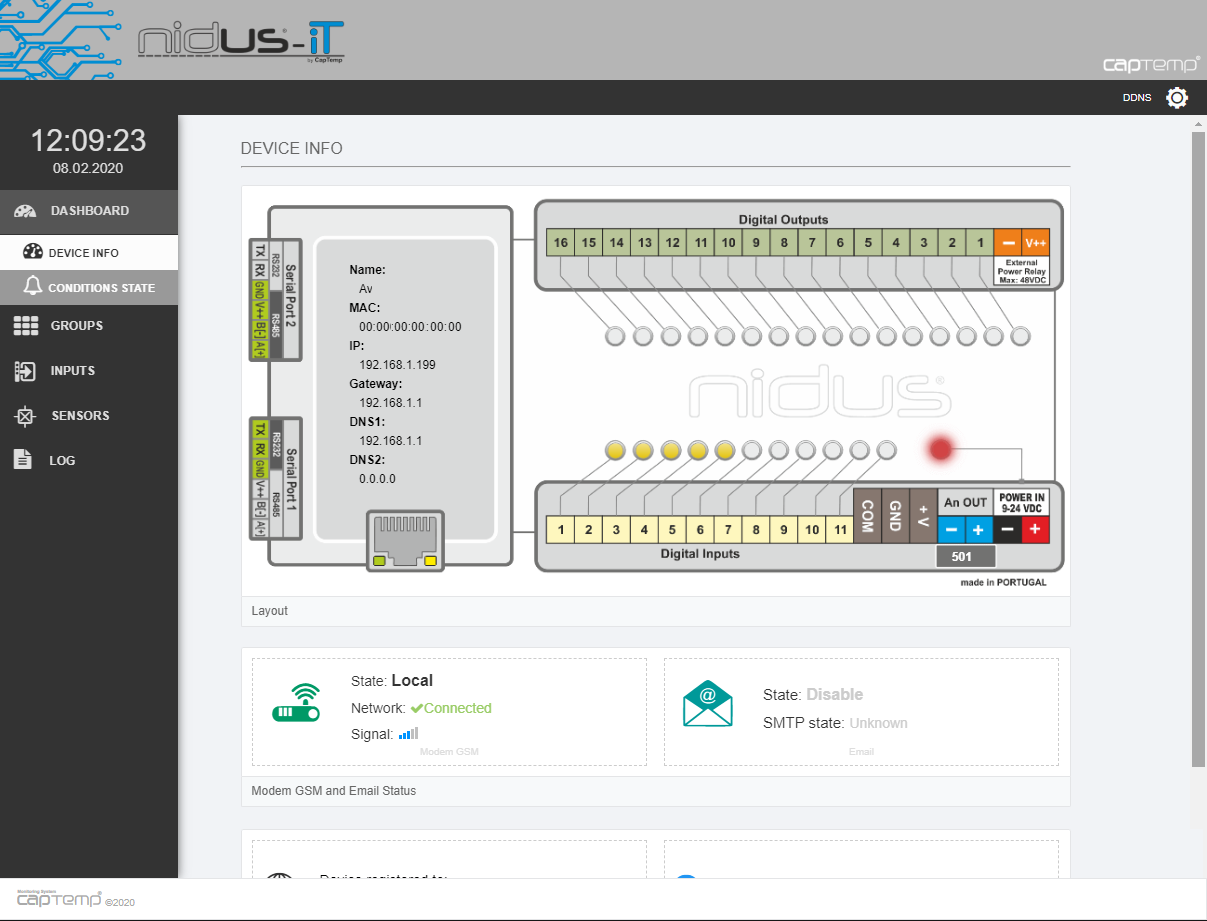
\includegraphics[width=0.75\textwidth]{images/layoutPAginaInit.png}
\caption{Layout página da Nidus IT no início do estágio}\label{fignidusPage}
\end{figure}


\section {NB-Iot \& Digi Xbee 3 }\label{nbiot}
\par
Os módulos Xbee 3 representado na figura \ref{figxbee} da DIGI dispõe recentemente de uma versão NB-Iot/ LTE. Ideal para projetos com baixo volume de transmissão de dados e com baixo consumo de energia. O módulo inclui também um compilador de Micropython, porém a versão Micropython desenvolvida pela DIGI e incluída no módulo XBee, não inclui todas as funcionalidades do Micropyhton tais como por exemplo a biblioteca de gestão de Arrays e o módulo de "\_thread" pois o mesmo não tem suporte para \textit{multithread}.
Na tabela \ref{tab1} são apresentadas as principais características do módulo XBee 3 da Digi\cite{Digixbee}.

\begin{figure}[ht]
\centering
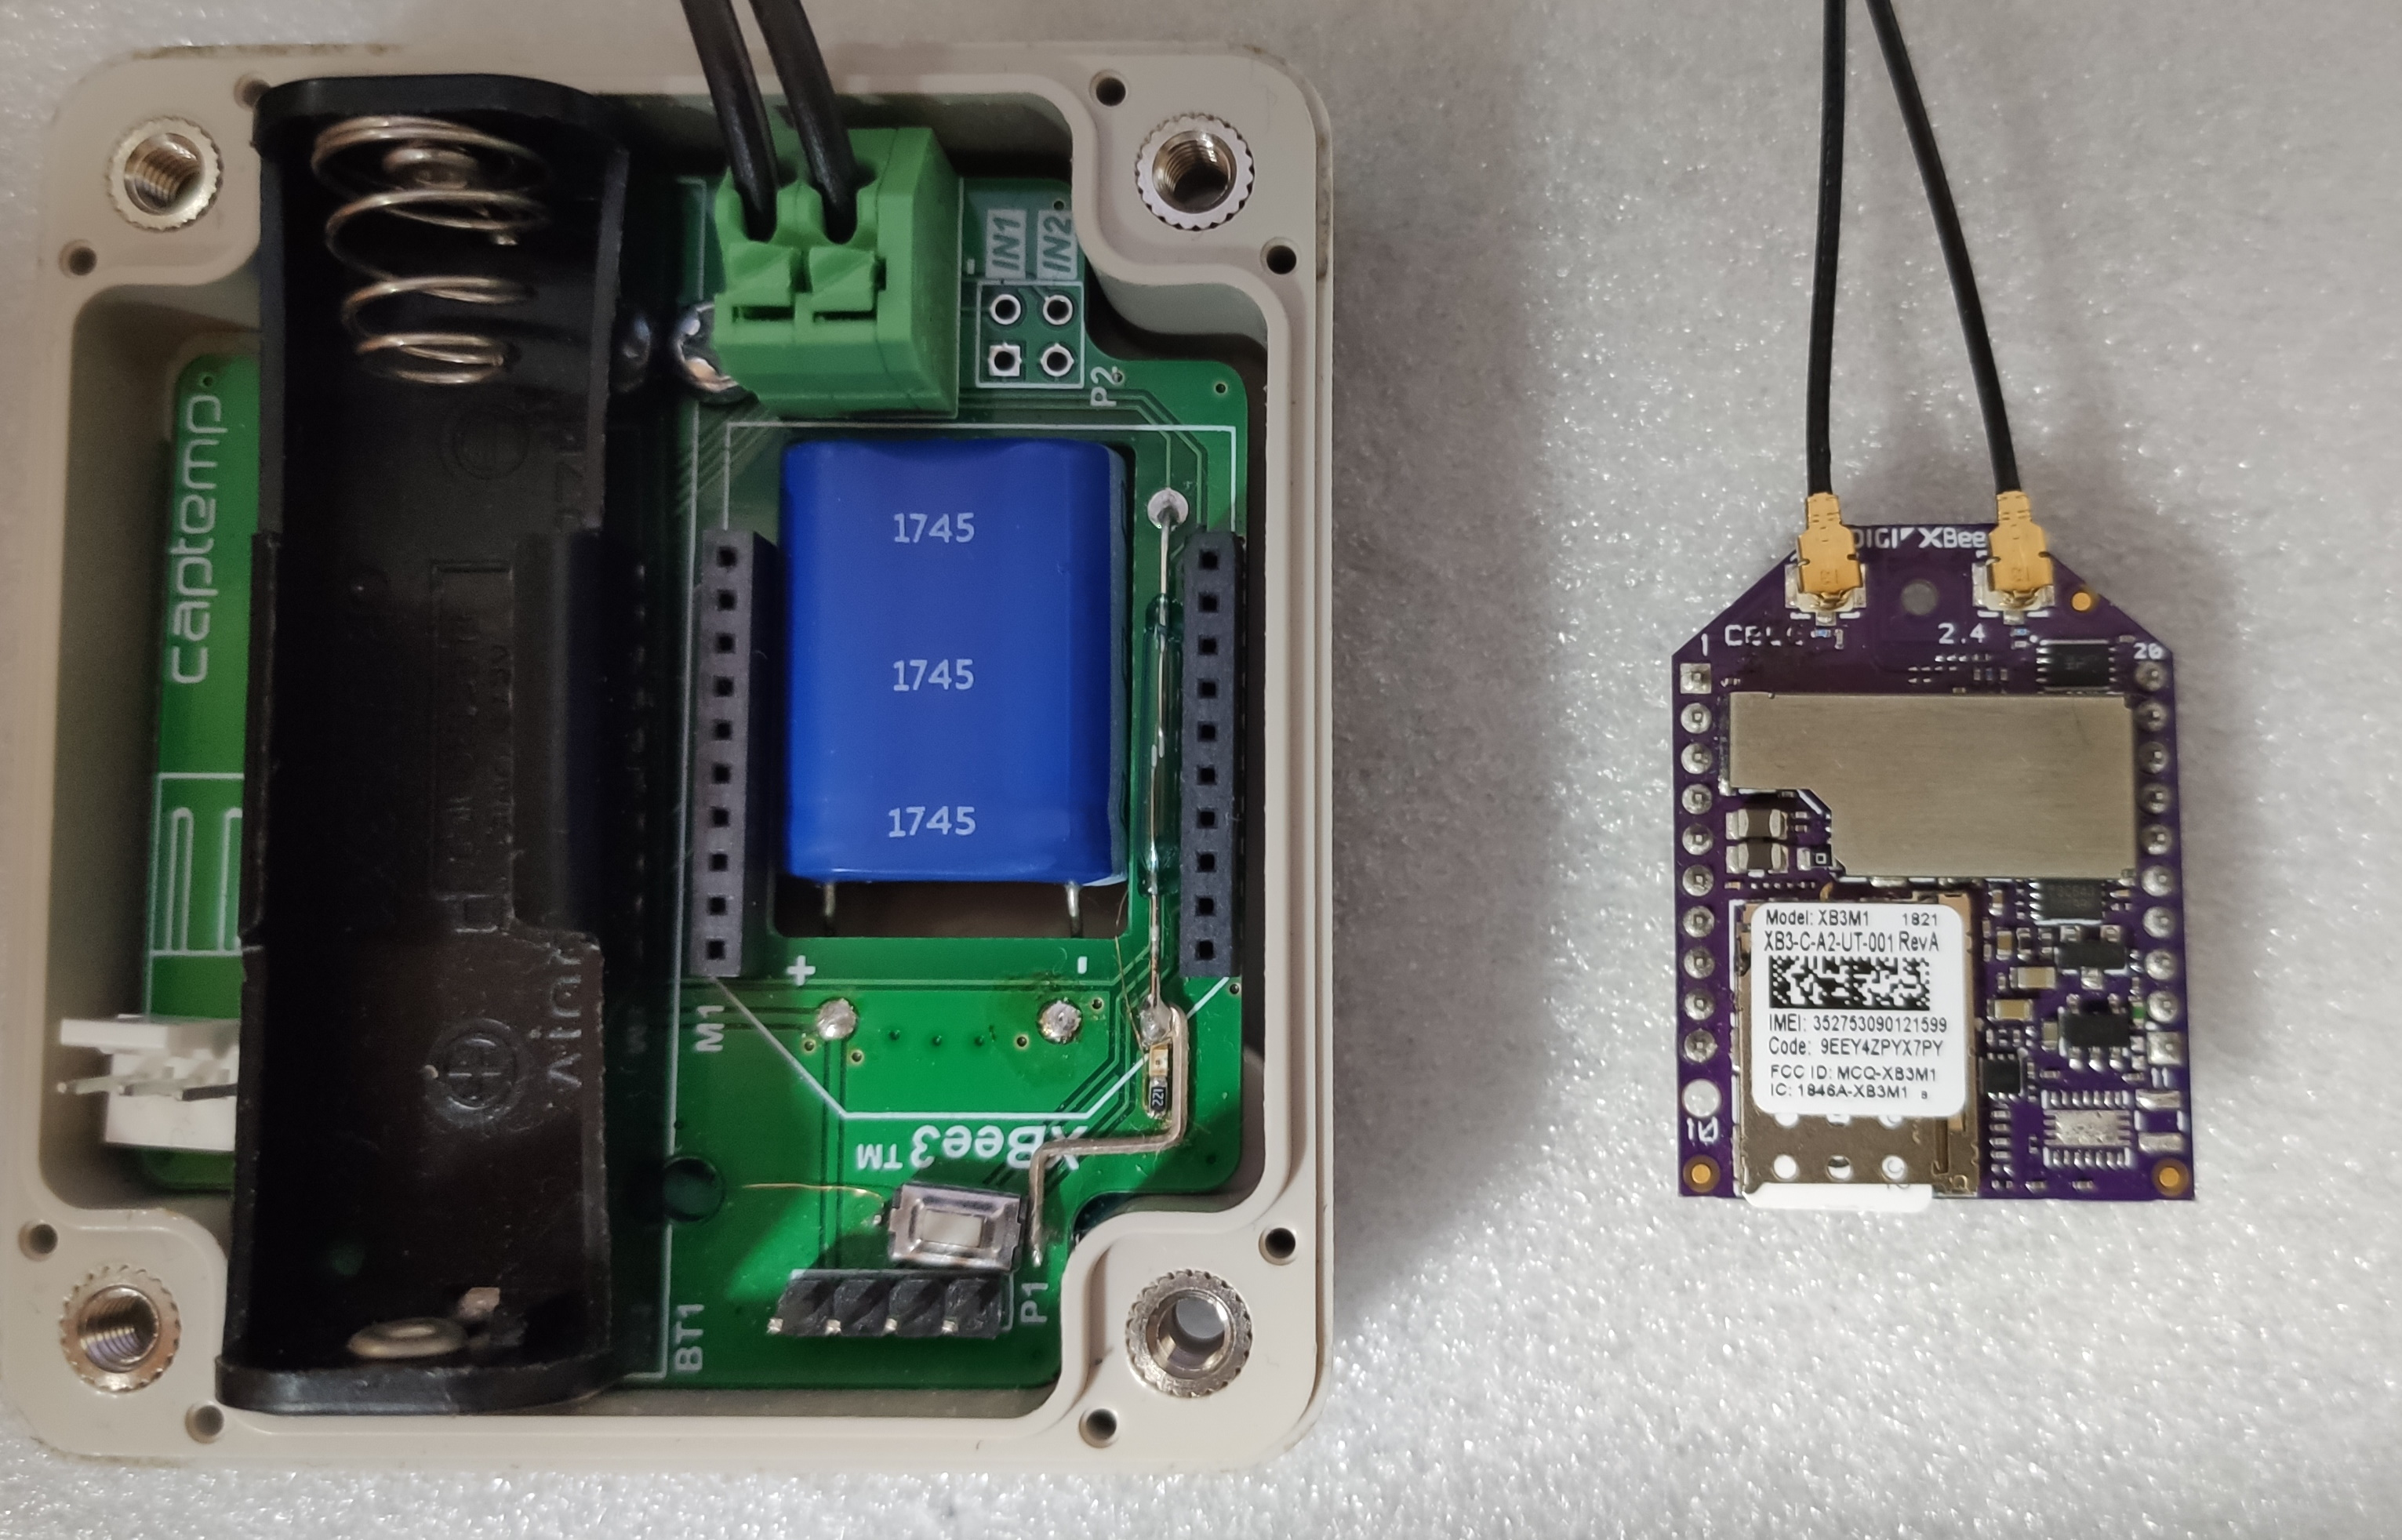
\includegraphics[width=0.60\textwidth]{images/xbee.jpg}
\caption{Módulo Xbee 3 e placa de expansão desenvolvida pela Captemp}\label{figxbee}
\end{figure}

\begin{table}[htb]
\caption{Especificações do Módulo Xbee 3}\label{tab1}
\begin{tabular}{|c|c|}\hline
Chipset& U-blox SARA-R410M-02B\\\hline
Dimensões& 24.38 mm x 32.94 mm \\\hline 
Temperatura de Funcionamento& -40º C to +85º C \\\hline 
Tipo de SIM & 4FF Nano \\\hline
Interfaces& UART, SPI, USB \\\hline 
Programação MicroPython& 32 KB Flash / 32 KB RAM \\\hline 
I/O& 4 ADC (10-bit), 13 I/O digitais, USB, I2C \\\hline 
Bluetooth& BLE Ready \\\hline 
Potencia de Transmissão& Até 23 dBm \\\hline 
Sensibilidade de Receção (LTE-M) & -105 dBm \\\hline 
Sensibilidade de Receção (NB-IoT) & -113 dBm \\\hline 
Velocidade Downlink/Uplink(LTE-M) & Até 375 kb/s \\\hline 
Velocidade Downlink/Uplink(NB-IoT) & Até 27.2 kb/s Downlink, 62.5kb/s Uplink \\\hline 
Alimentação & 3.3-4.3VDC \\\hline 
Pico corrente na transmissão & \begin{tabular}{@{}c@{}} 550mA - Bluetooth OFF \\ 610mA - Bluetooth ON\end{tabular}\\\hline 
Corrente média de transmissão (LTE-M) & 235mA \\\hline 
Corrente média de transmissão (NB-IoT) & 190mA \\\hline 
Modo Power Save& 20uA \\\hline 
Modo Deep Sleep& 10uA \\\hline 
\end{tabular} 
\end{table}

\par A Captemp pretende, através da utilização deste módulo e de uma placa de expansão desenvolvida pela própria, apresentada anteriormente na figura \ref{figxbee}, desenvolver uma versão do seu outro equipamento de Nb-Iot, mais simples representando numa opção de menor custo para o cliente. Será necessário desenvolver todo o código referente à gestão interna de Logs para guardar informação quando não existe cobertura para envio, o agendamento do envio e leituras, otimização da memória e bateria e implementação de comunicação bidirecional com encriptação com o portal Senslive. Sempre com recurso á programação em MicroPython.
A placa de expansão inclui um módulo de RTC, um conversor 1Wire para possibilitar a leitura de sondas já desenvolvidas pela Captemp, um sistema de alimentação para possibilitar a alimentação por pilha ou por alimentação externa. Ao desenvolver todo o equipamento a empresa tem o controlo total sobre o Firmware e sobre a estrutura de envio e a vantagem de tornar o equipamento compatível com todos os sensores que já possui.

\subsection {MicroPython}
\par O MicroPython\cite{MicroPython}, lançado em 2014, é um compilador e interpretador que implementa a linguagem Python3 e otimiza o seu funcionamento em microcontroladores. Escrito em C e disponibilizado em \textit{open-source} é possível adaptar o mesmo para os diversos equipamentos. \par
É suportado por diversas arquiteturas de processadores tais como:
\par
\begin{itemize}
\item x86
\item x86-64
\item ARM
\item ARM Thumb
\item Xtensa
\end{itemize}
\par
Em microcontroladores que suportem \textit{multi-thread} , não sendo o caso do módulo usado está disponível ao programador o módulo de "\_thread" para criar processamento paralelo. Disponibiliza a programação de interrupções físicas, uteis em microcontroladores, tem disponível um \textit{Garbage collector} para gerir a memória do microcontrolador e bibliotecas tais como "usocket" para criação e gestão de sockets, "network" para gerir a comunicação com o módulo específico de cada microcontrolador, ou a biblioteca para gerir o módulo de bluetooth denominada por "ubluetooth". As bibliotecas disponíveis encontram-se no site oficial da documentação\cite{micropython_lib}. 

\subsection {NB-Iot/ LTE-M}
O NB-Iot ou Narrowband Iot e o LTE-M são tecnologias de \textit{Low Power Wide Area}. São indicadas para sistemas \textit{smart} em diversas áreas como a monitorização, a agricultura, localizadores entre outras áreas. Similar ao funcionamento da rede móvel, onde cada equipamento possui um cartão SIM e se liga á rede fornecida pelo operador, mas utilizado em equipamentos com menor transmissão de dados e que não tem acesso a fontes de alimentação fixas e requerem de baterias, o NB-Iot promete autonomias das baterias a rondar os 10 anos\cite{u_2017}.Devido ao baixo volume de dados o plano de dados é possível apenas com pequeno investimento obter anos e até décadas de transmissões de dados.
\par De entre as vantagens podem-se destacar:
\begin{itemize}
\item Baixo consumo
\item Longo alcance e boa penetração
\item Baixo custo de desenvolvimento na implementação da cobertura
\item Custo reduzido pelas transmissões
\item Sem necessidade de Roaming
\end{itemize}
\par
A cobertura da rede está a ser implementada pelas operadoras de telecomunicações que já possuem cobertura da rede GSM e infraestrutura de ligação á rede Internet desenvolvida e apenas necessitam de 
disponibilizar cobertura nas antenas de rede móvel, normalmente já existe compatibilidade de \textit{Hardware} e basta atualizações de \textit{Firmware}. É aconselhado pelas operadoras que se utilize o Nb-Iot para equipamentos fixos e o LTE-M para equipamentos em movimento.

\subsubsection { Low Power Wide Area}
As redes \textit{Low Power Wide Area}, ou simplesmente denominadas por LPWAN são redes usadas frequentemente no IOT quando é necessário enviar dados a distâncias longas. Combinam a largura de banda e o consumo de bateria presente em redes como BLE e Zigbee, com alcance igual ou superior às redes de comunicação GSM. São caracterizadas por ter longo alcance, um baixo custo de transmissão e baixo consumo, onde simples baterias podem fornecer alimentação na ordem das décadas. Este alcance pode ser conseguido por exemplo por redes \textit{multihop} ou modulações especificas que privilegiem o consumo energético e o alcance. A comunicação 2G e 3G pode ser usada em comunicação M2M mas as mesmas tem uma largura de banda superior ao necessário o que resulta em consumo de bateria excessivo onde não é tirado proveito da largura de banda disponível. Alguns exemplos de redes LPWAN, são o DASH7, o SigFox, LoRa, Ingenu, Telensa ou o NarrowBand Iot.\cite{lpwanoverview}

\begin{figure}[ht]
\centering
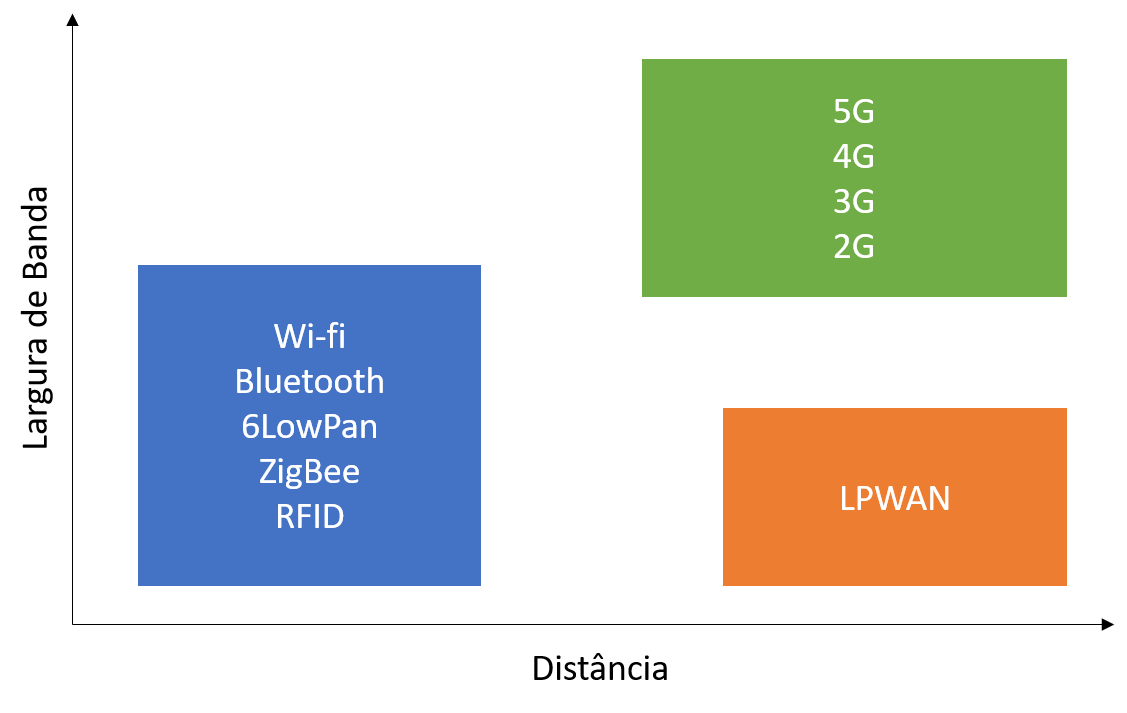
\includegraphics[width=0.45\textwidth]{images/lpwan.png}
\caption{Gráfico com relação Distancia vs Largura de Banda\cite{masterthesisLPWAN}}\label{figgraphlpwan}
\end{figure}



\section {Kea Tracker}\label{kea}
O Projeto Kea Tracker utiliza beacon’s da Ruuvi, uma beacon \textit{open-source}\cite{ruuvi}, que disponibiliza de forma \textit{open-source} tanto o \textit{Firmware} para alterações, como as aplicações para Android e IOS. Será desenvolvida uma aplicação baseada na aplicação fornecida e o \textit{Firmware} para disponibilizar a funcionalidade de data-logger.
\subsection{Beacons BLE}
\par
O \textit{Bluetooth Low Energy} ou simplesmente BLE foi desenvolvido a pensar nos novos equipamentos IOT, onde os utilizadores querem vários equipamentos ligado ao mesmo tempo. Para tal foi desenvolvido o BLE que permite mais ligações ao mesmo tempo comparando com o \textit{Bluetooth} clássico.
Como é indicado no nome, o principal fator diferenciador nesta versão, utilizada muitas vezes em equipamentos IOT, é o baixo consumo de aproximadamente metade relativamente ao \textit{Bluetooth} normal. Outras características melhoradas a visar os equipamentos de IOT no BLE são a baixa largura de banda e o baixo tempo de transmissão.

Com o desenvolver do BLE foram criados, novos tipos de equipamentos, nomeadamente as beacons, equipamentos quase sempre alimentados por pilhas, que comunicam através de BLE, tornando o equipamento portátil. As beacons são caracterizadas por transmitir pequenas quantidades de informação em \textit{broadcast}.
Existem dois tipos de beaco+++++ns, as beacons não conectáveis e as conectáveis\cite{blepacket}. Como indicado no nome as beacons conectáveis permitem que um equipamento (como um \textit{smartphone}) se conecte á beacons e esta fica preparada para receber dados. As não conectáveis apenas permitem o \textit{broadcast}  dos dados, poupando energia pois apenas é necessário ter o módulo acordado para fazer o \textit{broadcast} e o restante do tempo podem estar num estado \textit{sleep}. Na figura \ref{blepacket} é apresentado o pacote que é transmitido em \textit{broadcast} para os outros equipamentos ao alcance.

\begin{figure}[htb]
\centering
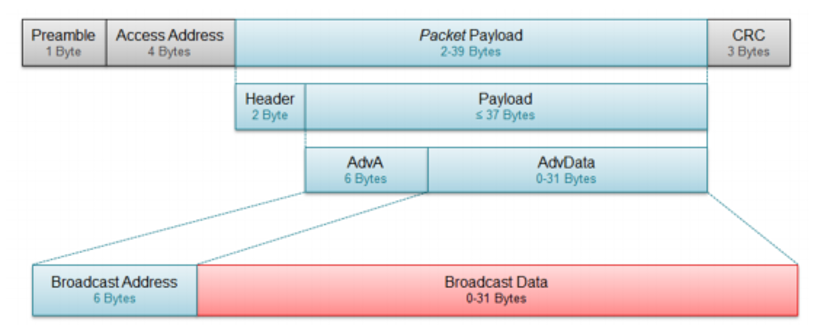
\includegraphics[width=0.65\textwidth]{images/blepacket.png}
\caption{\textit{BLE broadcast packet}\cite{blepacket}}\label{blepacket}
\end{figure}


\subsection{Ruuvi beacons}
\par Neste projeto o \textit{Firmware} das beacons necessita de uma alteração, tornar a beacon numa beacon conectável e esta armazenar internamente as últimas leituras num \textit{buffer} circular e criar um data-logger e caso o cliente pretenda poderá conectar mais tarde para fazer o \textit{download} para aplicação e posterior envio para o Senslive, não necessitando a proximidade do \textit{smartphone} á beacon durante todo o tempo. A Ruuvi dispõe de dois modos de desenvolvimento de \textit{Firmware} da beacon em C ou usando o Espruino, á semelhança do MicroPython um interpretador de JavaScript para microcontroladores lançado em 2012, totalmente compatível com as beacons da Ruuvi.

\subsection{Apps smartphones}
Na fase inicial será adaptada a versão disponibilizada para Android para agilizar a integração com o portal Senslive. Na segunda fase deste projeto será desenvolvida uma versão de raiz apenas com as funcionalidades necessárias. A aplicação base para android disponibilizada pela Ruuvi foi desenvolvida em Kotlin\cite{ruuviappgithub}, uma linguagem desenvolvida pela JetBrains multiplataforma e que inclui o Android nessas plataformas compatíveis.
De seguida estão apresentadas as alterações necessárias na aplicação já existente:
\begin{itemize}
\item Alteração das imagens e logotipo da app;
\item Alteração do nome da App;
\item Remoção de conteúdo não necessário;
\item Bloqueio do URL de envio para usar exclusivamente o portal Senslive;
\item Melhoramento da precisão da posição GPS;
\item Possibilidade da alteração dos intervalos de registo
\item Leitura dos registos dos equipamentos
\end{itemize}



\section{dot.Tracker} \label{dot.tracker}


\par O Projeto dot.Tracker é um desenvolvimento de um projeto a pedido do cliente que pretende através de uma plataforma WEB monitorar a posição de objetos e de pessoas em tempo real. Neste projeto serão utilizadas beacons BLE e \textit{Gateways} responsáveis por receber os pacotes das beacons e os transmitir para um servidor. O servidor será capaz de processar os pacotes e calcular a posição da beacon no mapa e informar os utilizadores sobre alertas e estatísticas. Visto este projeto ter sido solicitado por um cliente que pretendia uma solução à medida e este não se encontrar no espaço Europeu não há problemas de registo e armazenamento do \textit{Tracking} das pessoas devido á legislação em vigor na Europa para proteção de dados, o RGDP.

Á semelhança do projeto Kea Tracker o projeto dot.Tracker usa igualmente beacon's BLE para enviar a informação necessária para o respetivo portal. É necessário recolher os pacotes recebidos das beacons enviá-los para o servidor e calcular a distância entre a beacon e o recetor e com o auxilio de múltiplos recetores realizar a triangulação da beacon num mapa. No decorrer do projeto será necessário desenvolver uma plataforma WEB para receber e visualizar as localizações provenientes das beacons e respetivas configurações, adotar o método de algoritmo para a triangulação da beacon relativamente a vários recetores e realizar testes ao funcionamento e precisão do sistema.
\subsection{Beacons e \textit{Gateway}}
Para este projeto irá ser utilizado durante o desenvolvimento a solução da Beacon Line\cite{taskit} e outras a pesquisar de modo a procurar as melhores soluções e posteriormente desenvolvido recetores proprietários da Captemp. A solução apresentada pela Beacon Line, é composta por um \textit{Gateway} e vários nós. Cada nó possui um recetor BLE e quando o mesmo recebe um \textit{broadcast} proveniente da beacon o transmite para o \textit{Gateway}. Caso exista alguma divergência da potência de transmissão desde o último pacote enviado por essa mesma beacon o gateway com conectividade Ethernet realiza o \textit{Publish} num broker onde é possível o servidor obter os pacotes das beacon's. As restantes soluções baseiam-se em equipamentos com uma interface BLE e outra Wi-Fi e comunicam diretamente com o servidor ao invés de comunicarem com um ponto central como acontece no caso da Beacon Line.


\section{Soluções e tecnologias disponíveis} \label{solucoesDisponiveis}

Neste subcapítulo é abordado algumas das abordagens possíveis para atingir os objetivos nas secções anteriores (Secção \ref{compressaoFicheiros}), assim como a aplicação dos mesmos em produtos existentes (Secção \ref{produtos}).


\subsection{Tecnologias disponíveis} \label{compressaoFicheiros}

Existem diversas abordagens possíveis para a compressão de ficheiros de código, de imagens e localização \textit{indoor}. Algumas destas são descritas de seguida.

\subsubsection{Compressão de ficheiros} 
\par
Atualmente a vida \textit{online} do Homem passou a ter um grande impacto na sua vida. Para tal as páginas WEB e seus conteúdos foram aumentado em quantidade e tamanho e com menores tempos de resposta. Isso é aplicável tanto aos ficheiros que contem o layout da página, quer das imagens. Para poupar dados de transmissão e reduzir tempos de envios, ou simplesmente suportar larguras de banda inferiores, os \textit{browsers} integraram a possibilidade de receber os ficheiros comprimidos e fazer a descompressão para mostrar ao cliente quase em tempo real. Atualmente os \textit{browsers} recentes suportam a compressão por GZIP( já utilizado na página do equipamento Nidus) e compressão utilizado a codificação Brotlin \cite{Alakuijala2019} \cite{brotlirfc}.
Cada método de compressão possui as suas vantagens e desvantagens, o brotli por sua vez á semelhança de outros métodos em comparação com o GZIP, tem uma taxa de compressão superior\cite{Alakuijala2015}, isto significa que consegue reduzir o mesmo ficheiro no seu respetivo ficheiro comprimido ocupando menos espaço em relação ao GZIP, mas como desvantagem o tempo de compressão do mesmo é superior. Ao contrário da compressão, na descompressão o Brotli tem melhores resultados do que nas restantes alternativas apresentando velocidades superiores de descompressão.
\par
O GZIP e o brotli usam na sua compressão para reduzir o tamanho do ficheiro o algoritmo de compressão LZ77, que procura sequências repetidas utilizando o método de janela deslizante e substitui essas sequências por referências para a primeira ocorrência que não foi substituída indicando a distância a que a primeira ocorrência ocorre e o tamanho a substituir.
\par O sistema de janela deslizante define um tamanho da janela e ao deslocar a janela do tamanho definido define um dicionário. Após definir o dicionário com vários tamanhos de janelas, percorrer novamente o ficheiro através do método de janela deslizante novamente a procurar repetições das entradas que existem no dicionário. Quando uma sequência é encontrada esta é substituída por uma referência da posição da primeira ocorrência da mesma. Na figura \ref{janela} é apresentado um exemplo do funcionamento da janela deslizante para a obtenção do dicionário com o tamanho da janela a variar de 2 a 7.
\begin{figure}[htb]
\centering
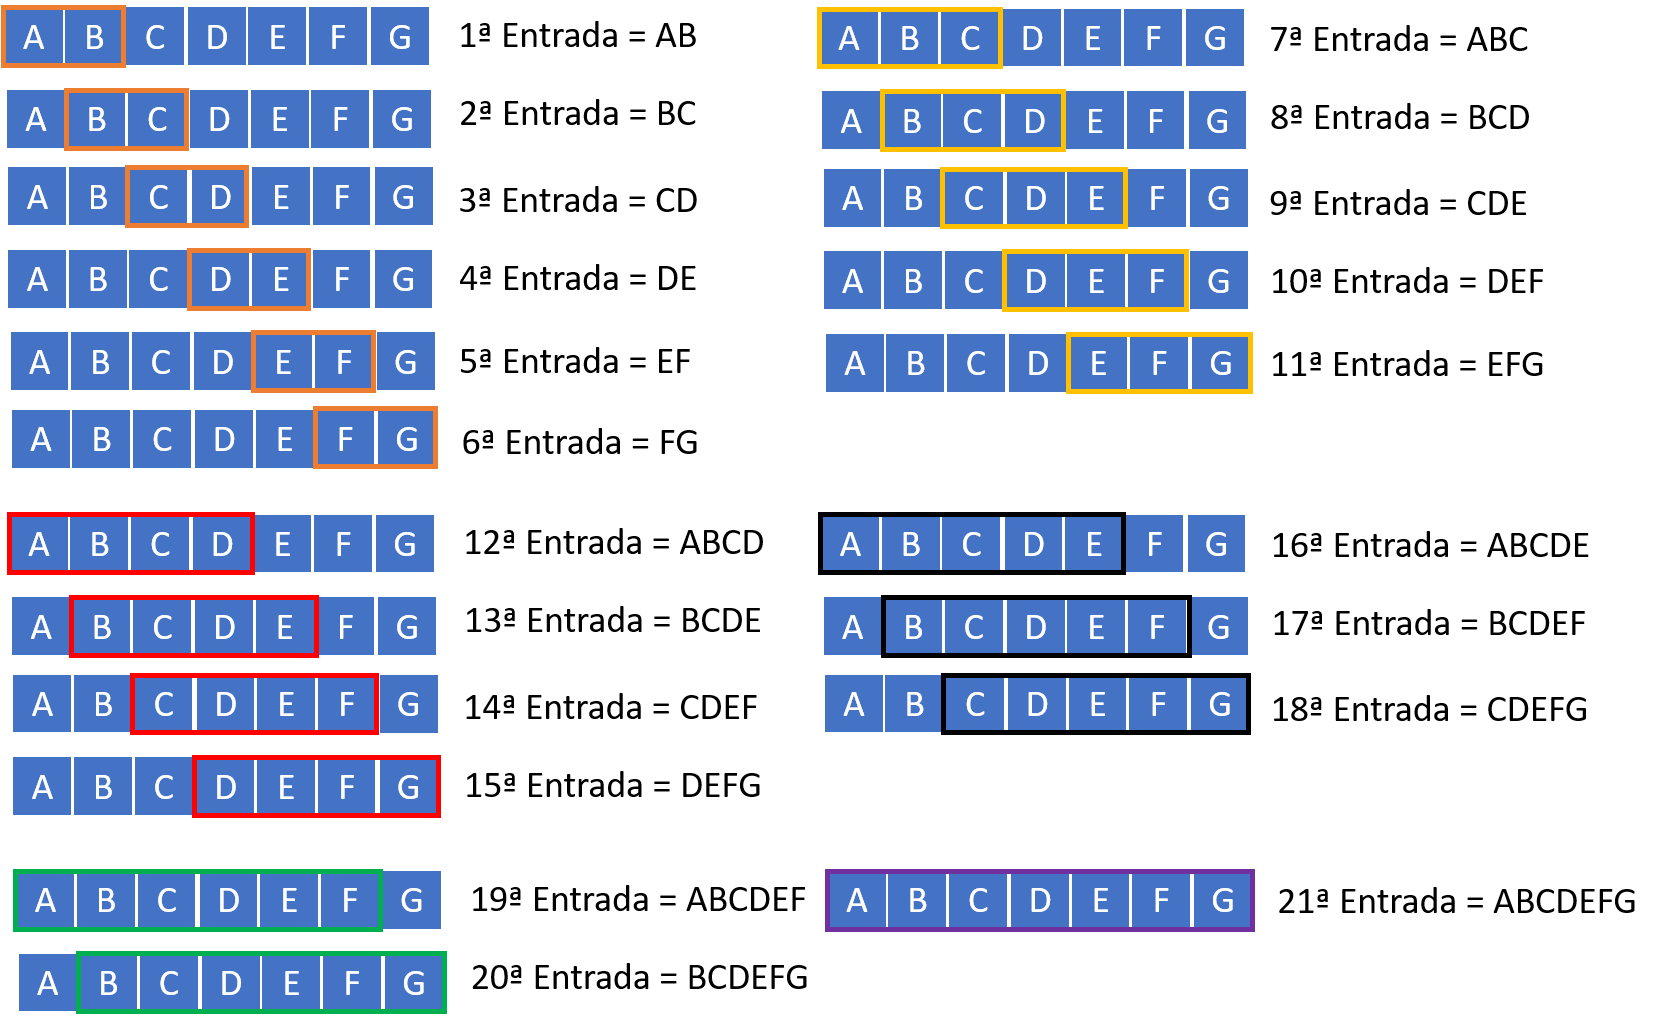
\includegraphics[width=0.85\textwidth]{images/janeladeslizantedicionario.png}
\caption{Funcionamento da Janela Deslizante}\label{janela}
\end{figure}


\par Na figura \ref{gzip} e \ref{gzip2} é apresentado dois exemplos visuais e simples utilizando frases de como o LZ277, usado pelo GZIP e Brotl através do sistema de janela deslizante procura as repetições e comprime os ficheiros. Na Figura \ref{unzip} é apresentado o ficheiro base, representado por um pequeno texto. No exemplo apresentado pela figura \ref{gzip} apenas foi utilizado a substituição de palavras inteiras, na figura \ref{gzip2} procura sequências de caracteres sejam elas palavras ou não. Nos exemplos apresentados a redução foi de 20\% [$1-\dfrac{48}{60}\times100\%$] no primeiro exemplo e de aproximadamente de 32\% [$1-\dfrac{41}{60}\times100\%$] no segundo.
\begin{figure}[htb]
\centering
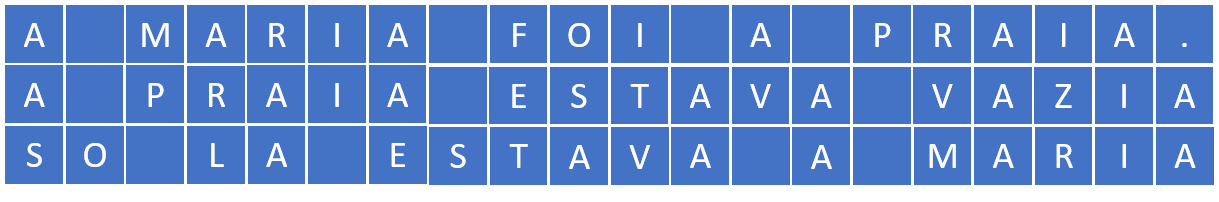
\includegraphics[width=0.85\textwidth]{images/FILE.png}
\caption{Sequência não comprimida}\label{unzip}
\end{figure}

\begin{figure}[htb]
\centering
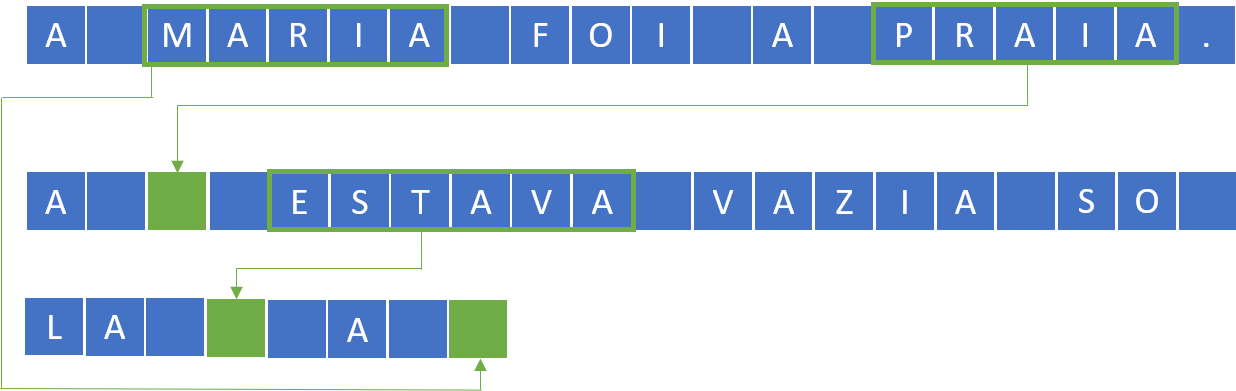
\includegraphics[width=0.85\textwidth]{images/gzip.png}
\caption{Sequência comprimida com LZ77 (apenas palavras)}\label{gzip}
\end{figure}
\begin{figure}[htb]
\centering
\includegraphics[width=0.85\textwidth]{images/gzip2.png}
\caption{Sequência comprimida com LZ77(palavras e sequências)}\label{gzip2}
\end{figure}




\subsubsection{Compressão de imagens}
\par

O utilizador pretende igualmente ver as imagens com a máxima qualidade, mais qualidade significa um maior detalhe e por sequencia um ficheiro de maior tamanho. Existem atualmente vários \textit{softwares online} e locais que reduzem o tamanho das imagens. Na conceção da página da Nidus é utilizado o \textit{website} TinyPNG.com que analisa a imagem original e converte as cores em cores mais simples de o sistema armazenar, como por exemplo uma imagem com 24 bits de profundidade de cor, onde cada cor é representada por 24 bits pode ser convertido em uma similar com apenas 8 bits reduzindo o tamanho do ficheiro e impercetível para o olho humano num ecrã digital\cite{Hilles2019}. Alternativamente ao Tiny Png existem \textit{softwares}, similares alguns de licença GNU/GPL, para comprimir imagens. Com o "Mass Image Compressor"\cite{Mass_Image_Compressor}(apenas um exemplo), é possível comprimir as imagens com a possibilidade de indicar a quantidade de compressão.
\par
Com a enorme quantidade e diversidade de monitores existentes, as páginas web necessitam de ser responsivas e apresentar a melhor imagem para o monitor em questão, isso normalmente traduz-se em várias versões similares da imagem alojadas no servidor. No caso dos microcontroladores e sistemas embebidos o espaço encontra-se limitado e deve-se arranjar uma solução. Uma solução possível é ao invés da utilização de imagens PNG, JPG ou outras, é a utilização de imagens em SVG, onde a imagem é representada por um ficheiro XML que descreve uma imagem bidimensional e utiliza na sua constituição modelos matemáticos para o cálculo das posições dos elementos. Com isto é possível manipular o XML em tempo real para alterar elementos ou remover, alterar cores, criar animações entre outras. Inclui a vantagem de como a imagem é representada por formulas matemáticas, é possível escalar a imagem sem perder qualidade, pois a função matemática é ajustável. Num sistema embebido como o caso da Nidus é vantajoso a utilização de imagens em SVG para criação das animações. Atualmente as animações da página da Nidus são criadas com várias imagens PNG comprimidas e convertidas em base64 e são alternadas no HTML pelo JavaScript. Com a utilização de imagens SVG é possível ter apenas uma imagem alojada e manipular a imagem em tempo real através do JavaScript de uma forma mais suave para o utilizador, pois apenas a zona a alterar é alterada na imagem.
Á semelhança dos JPG e PNG o SVG também pode ser comprimido, para tal basta no XML da imagem remover os meta-dados e utilização de funções matemáticas mais simples, não necessários para o browser apresentar a representação gráfica do mesmo, mas os \textit{softwares} de edição adicionam para funcionalidades exclusivas do editor. Á semelhança dos ficheiros HTML após a remoção dos meta-dados o ficheiro pode ser minificado.

\subsubsection{Localização \textit{indoor}} \label{indoor}
\par
É possível encontrar na comunidade científica vários estudos sobre a utilização de redes Wi-Fi e Bluetooth para sistemas de localização. Estes mesmos focam-se no cálculo das distâncias do equipamento para vários recetores no mesmo intervalo temporal, algumas destas soluções baseiam-se nos valores de RSSI da transmissão e o valor definido como constante da potência de transmissão á distância de 1 metro, e estimar a sua distância aproximada de cada recetor, com essas aproximações é possível através do algoritmo escolhido\cite{Wang2013}, obter a estimativa da localização do equipamento e a sua colocação num mapa.
A distância de um recetor para o emissor baseada no valor de RSSI é expressa pela seguinte fórmula, onde dbm é a constante da potência de transmissão da beacon a 1 metro, n a constante do ambiente e o RSSI corresponde ao RSSI da transmissão:
\par
\begin{center}
$d=10^(\frac{dbm-RSSI}{10 \times n})$
\end{center}

\par
Após a obtenção da distância para cada recetor é possível aplicar um algoritmo para estimar a localização. Os mais referenciados e adotados são o \textit{centroid} baseado no centro geométrico do polígono formado pelas interceções das circunferências criadas com o raio da distância calculada pela fórmula anteriormente apresentada, o método \textit{Three-border Positioning} e o \textit{Least Square Estimation}.
Como é possível observar na figura \ref{centroid} utilizando o método \textit{centroid}, o centro geométrico corresponde á localização do equipamento com base nos recetores. A fórmula que representa o centro utilizando o \textit{centroid} é expressa pela seguinte equação onde n representa o numero de recetores utilizados no cálculo.
\par
\begin{center}
$ (x,y)= (\frac{x_{1}+x_{2}+x_{3}+...+x_{n}}{n},\frac{y_{1}+y_{2}+y_{3}+...+y_{n}}{n})$
\end{center}

\begin{figure}[htb]
\centering
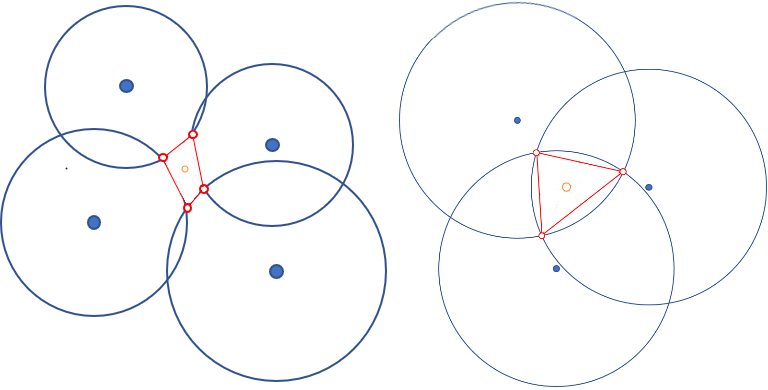
\includegraphics[width=0.95\textwidth]{images/centroid3.png}
\caption{Posição utilizando o método \textit{Centroid} com 3 e 4 recetores}\label{centroid}
\end{figure}

Ao invés da utilização do método do \textit{centroid} se for adotado o método \textit{Three-border Positioing}, é criada a função definida por ramos composta pelas três equações da circunferência A, B e C com os respetivos centros em cada recetor e com o raio igual á distância calculada para esse mesmo recetor. Para calcular a posição estimada é calculado o resultado dessa mesma função de modo a encontrar o ponto x,y que representa a posição do equipamento.
\par 
Utilizando o método \textit{Least Sqare Estimation} ou simplesmente LSE e á semelhança do Three-border Position\cite{Zhu2014} é criada a função de ramos das equações das circunferências dos vários recetores com o raio da distância calculada, mas pode igualmente como o \textit{centroid} utilizar mais do que três recetores aumentando a precisão. \par Hua, Z., Hang, L., Yue, L., Hang, L., \& Kan, Z. (2014). Geometrical constrained least squares estimation in wireless location systems. 2014 4th IEEE International Conference on Network Infrastructure and Digital Content. apresenta os passos necessários calcular a posição X do equipamento através do método LSE. Em primeiro são criadas a função de ramos composta pelas equações das circunferências com centro nos recetores ([$x_{1}$,$y_{1}$],[$x_{2}$,$y_{2}$],[$x_{3}$,$y_{3}$],[$x_{4}$,$y_{4}$]) e o raio igual á distância calculada($d_{1}$,$d_{2}$,$d_{3}$,$d_{4}$).
\begin{center}
\[
\begin{cases}
(x_{1} -x)^2 + (y_{1}-y)^2 = {d_{1}}^2\\
(x_{2} -x)^2 + (y_{2}-y)^2 = {d_{2}}^2\\
(x_{3} -x)^2 + (y_{3}-y)^2 = {d_{3}}^2\\
(x_{4} -x)^2 + (y_{4}-y)^2 = {d_{4}}^2\\
\end{cases}
\]
\end{center}

\par Após a criação da função é subtraído o primeiro ramo aos restantes ramos e a função reduz o numero de ramos para n-1 onde n representa o numero de recetores a usar na função.
\begin{center}

\[
\begin{cases}
2(x_{2}-x_{1})x+2(y_{2}-y_{1})y={x_{2}}^2-{x_{1}}^2+{y_{2}}^2-{y_{1}}^2+{d_{2}}^2+{ d_{1}}^2\\
2(x_{3}-x_{1})x+2(y_{3}-y_{1})y={x_{3}}^2-{x_{1}}^2+{y_{3}}^2-{y_{1}}^2+{d_{3}}^2+{ d_{1}}^2\\
2(x_{4}-x_{1})x+2(y_{4}-y_{1})y={x_{4}}^2-{x_{1}}^2+{y_{4}}^2-{y_{1}}^2+{d_{4}}^2+{ d_{1}}^2\\
\end{cases}
\]
\end{center}
\par A função pode ser representada pelo seu equivalente numa representação de matrizes por $2AX = b$ onde.

\begin{center}



$A=\begin{bmatrix}
x_{2}-x_{1} & y_{2}-y_{1}\\
x_{3}-x_{1} & y_{3}-y_{1}\\
x_{4}-x_{1} & y_{4}-y_{1}
\end{bmatrix}$

$B=\begin{bmatrix}
b_{1}\\
b_{2}\\
b_{3}
\end{bmatrix}=\begin{bmatrix}
{x_{2}}^2-{x_{1}}^2 + {y_{2}}^2-{y_{1}}^2 - {d_{2}}^2 + {d_{1}}^2 \\
{x_{3}}^2-{x_{1}}^2 + {y_{3}}^2-{y_{1}}^2 - {d_{3}}^2 + {d_{1}}^2 \\
{x_{4}}^2-{x_{1}}^2 + {y_{4}}^2-{y_{1}}^2 - {d_{4}}^2 + {d_{1}}^2 \\
\end{bmatrix} $

\end{center}

\par A posição estimada do equipamento representada no exemplo por X é definida por:



\par
\begin{center}
$ X= \frac{1}{2}(A^T A)^{-1} A^T b$
\end{center}

\par Os testes analisados demonstram\cite{Wang2013} , que o método LSE é o método que obtém os melhores resultados com os valores mais próximos do real. No teste apresentado em segundo lugar está o \textit{Three-border Position} e por último o \textit{centroid}. Com algumas discrepâncias em algumas das amostragens.

\subsection{Produtos similares} \label{produtos}

\par Neste subcapítulo é abordado alguns produtos já existentes no mercado para os projetos NB-IOT e Kea Tracker
\subsubsection{NB-Iot}
\par
Atualmente no mercado começam a surgir alguns produtos similares ao que se pretende desenvolver como é o caso dos sensores da Efento\cite{epoka}, que disponibiliza vários tipos de sensores que comunicam por NB-Iot. A Efento é uma empresa fundada em 2014 e é focada em desenvolvimento de equipamentos IOT. Atualmente desenvolveram versões com suporte para NB-Iot. Estes equipamentos tem a desvantagem de não ser compatível com o pacote de envio desenvolvido no portal Senslive e apenas permite o envio para o portal da Efento e não existe a possibilidade da utilização das sondas já comercializadas pela Captemp. Como vantagem á semelhança do equipamento a desenvolver é a utilização de um sistema com Log para quando não existe possibilidade de comunicação.
Devido ao desenvolvimento da tecnologia ainda existem poucas soluções em comercialização, estando as mesmas em desenvolvimento. A Captemp possui igualmente outro equipamento, completamente desenvolvido pela empresa, em desenvolvimento que tira partido do NB-Iot com o acréscimo em relação ao que se pretende desenvolver durante o estágio, a possibilidade de ter mais sensores, maior capacidade de Log interno, configuração por Bluetooth, GPS e um Display integrado como extras.


\subsubsection{Kea Tracker}
Após pesquisas \textit{online} é possível encontrar algumas soluções de beacons que permitem o armazenamento interno de leituras para desenvolver um sistema de data-logger tais como a beacon da Fujitsu, a FWM8BLZ02A-109069\cite{beacon1} , á semelhança da beacon da Ruuvi usa o mesmo chip o nRF52832 da Nordic Semiconductor, mas apresenta como vantagens a inclusão de um sistema de Logs interno com capacidade para aproximadamente 4080 leituras e a diversidade de sensores já incluídos. Como desvantagem em relação á beacon da Ruuvi tem a inclusão de um sensor de temperatura ao invés de temperatura e humidade, não possui sensor de pressão atmosférica e não é open-source possuindo um firmware fechado. A vantagem de se desenvolver um produto desde a sua raiz é a possibilidade de ter o controlo total sobre a solução para posteriores melhoramentos e ter a solução a desempenhar apenas o que pretendemos.
\par
Outra solução existente no mercado é igualmente a solução da Blue Maestro que possui variadas versões de beacons. Á semelhança da beacon da Fujitsu possuem igualmente sistema de Log. Contrariamente á FWM8BLZ02A-109069 é uma beacon que tem disponível em \textit{open-source} uma API e um SDK para desenvolver as nossas aplicações. Comparada com a beacon da Ruuvi, a Ruuvi beacon é completamente \textit{open-source} e não apenas a API para comunicação.
\par
Na tabela \ref{tabbeacons} são apresentadas as diferenças e semelhanças entre os três modelos analisados

\begin{table}[htb]
\caption{Comparação entre beacons \cite{specsrect}\cite{bluespecs}\cite{ruuvispecs}}\label{tabbeacons}
\begin{tabular}{|c|c|c|c|}\hline
& Ruuvi Tag& Fujitsu Beacon &Blue Maestro \\\hline
Processador& nRF52832& nRF52832 &? \\\hline
Memória&\begin{tabular}{@{}c@{}}512kB Flash \\ 64kB RAM\end{tabular} & 32K Não volátil &?\\\hline 
Protocolos&\begin{tabular}{@{}c@{}c@{}@{}c@{}} Bluetooth 5 \\ Wirepass \\ Mira OS\\QUUPA\\Others (2.4GHz)\end{tabular}&Bluetooth 4.1&BLE 4.2\\\hline 
\begin{tabular}{@{}c@{}}Potência de\\ Transmissão\end{tabular} &+4 dBm &\begin{tabular}{@{}c@{}}-16, -12, -8\\ -4, 0, +4 dBm\end{tabular} &-4, 0, +4 dBm \\\hline
Sensores& \begin{tabular}{@{}c@{}c@{}c@{}} Acelerometro\\ Temperatura\\ Humidade \\Pressão\end{tabular} &\begin{tabular}{c@{}c@{}} Acelerómetro\\ Temperatura\end{tabular}&\begin{tabular}{@{}c@{}c@{}} Temperatura\\ Humidade \\Pressão\end{tabular}\\\hline 
NFC & \checkmark&- &-\\\hline
Bateria &\begin{tabular}{@{}c@{}}CR2477\\ 1000mAH - Li/MnO2\end{tabular}&CR2450 &CR2032\\\hline
\begin{tabular}{@{}c@{}}Autonomia\\(espetável)\end{tabular}& ~10 Anos&1 Ano em Broadcast &\begin{tabular}{@{}c@{}}1 Ano em Broadcast\\2 Anos com Log\end{tabular}\\\hline
Data Logger &\begin{tabular}{@{}c@{}}-\\(a desenvolver)\end{tabular}&\checkmark &\checkmark\\\hline
Open Source & \checkmark&- &\checkmark ( API \& SDK )\\\hline
Informações & \begin{tabular}{@{}c@{}c@{}@{}} IP67 \\ 2 Botões\\2 Leds\\52mm \diameter\\\end{tabular}&\begin{tabular}{c@{}c@{}} Led\\ 40 x 31 x 12mm \end{tabular}&\begin{tabular}{@{}c@{}}24000 Registos\\33mm \diameter\end{tabular} \\\hline
\end{tabular} 
\end{table}
\par
